\section{Web-app amministratori}
\subsection{Introduzione}
La web app costituisce l'interfaccia tramite la quale l'amministratore può interagire col sistema.
Le funzionalità offerte sono:
\begin{itemize}
	\item login e logout;
	\item visualizzazione delle stanze e delle postazioni con i relativi stati;
	\item aggiunta, rimozione e modifica di stanze e postazioni;
	\item impostazione di postazioni come guaste;
	\item impostazione di stanze come inaccessibili;
	\item visualizzazione delle credenziali degli utenti;
	\item aggiunta, rimozione e modifica di credenziali;
	\item visualizzazione e scaricamento report sulle occupazioni e sulle igienizzazioni;
	\item visualizzazione di notifiche riguardanti il salvataggio dei dati sulla blockchain.
\end{itemize}

\subsection{Requisiti e installazione}
Il codice sorgente della web-app è pubblicato su GitHub all'indirizzo \url{https://github.com/DPCMGroup/bc19-webapp}.
Lo si può scaricare compresso in formato zip direttamente dal sito o, se si ha già installato il programma git, eseguendo il comando
\begin{verbatim}
	git clone https://github.com/DPCMGroup/bc19-webapp
\end{verbatim}

\subsubsection{Linguaggi}
\paragraph{Typescript}
Superset del linguaggio Javascript.

\paragraph{HTML}
Linguaggio di markup utilizzato per definire la struttura delle pagine web.

\paragraph{CSS}
Linguaggio per la definizione dello stile grafico delle pagine web.

\subsubsection{Tecnologie}
\paragraph{Node.js}
Programma focalizzato sull'esecuzione di codice javascript al di fuori del browser.
Per l'installazione fare riferimento alla pagina \url{https://nodejs.org/en/download/} 
\paragraph{npm}
Acronimo di Node Package Manager, permette di ottenere le librerie necessarie allo sviluppo.
Si ottiene insieme a Node.js tramite l'installazione di quest'ultimo.
\paragraph{Angular}
Framework per applicazioni web.
Per l'installazione fare riferimento alla pagina \url{https://angular.io/guide/setup-local#install-the-angular-cli}
\paragraph{Bootstrap}
Framework per la creazione di pagine web.
Per l'integrazione di bootstrap in angular fare riferimento alla pagina \url{https://www.npmjs.com/package/@ng-bootstrap/ng-bootstrap#installation}

\subsubsection{Test}

\subsection{IDE}
Per lo sviluppo abbiamo utilizzato l'IDE WebStorm. Per la sua installazione riferirsi alla pagina \url{https://www.jetbrains.com/webstorm/download/}

\subsection{Architettura}
L'architettura della web-app segue il modello a componenti imposto da Angular, che, a sua volta, si basa sul pattern Model-View-ViewModel, descritto dall'immagine sottostante.
\begin{figure}[H]
	\centering
	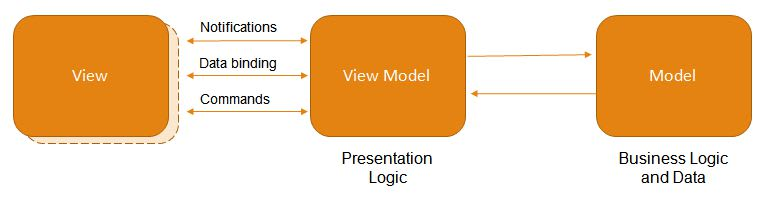
\includegraphics[width=15cm]{res/images/mvvm.jpg}
	\caption{Model-View-ViewModel}
	\label{fig:Model-View-ViewModel}
\end{figure}
Secondo questo modello la parte visiva del sito viene suddivisa in componenti, e ognuna di queste parti viene controllata da una diversa classe.
La parte visiva viene chiamata view, mentre la parte di controllo viene chiamata view model.
Un componente è costituito da 4 file. Nel seguente esempio è rappresentato un componente chiamato base.
\begin{verbatim}
	base.component.css
	base.component.html
	base.component.test.ts
	base.component.ts
\end{verbatim}
I file contengono, nell'ordine:
\begin{itemize}
	\item lo stile grafico del componente definito in css;
	\item la struttura del componente definito in html;
	\item i test definiti per il componente, scritti in typescript;
	\item il codice che definisce la logica del componente, scritto in typescript;
\end{itemize}

La struttura del sito è definita principalmente dal modo nel quale i componenti vengono annidati l'uno dentro all'altro. Nel codice html questo annidamento è descritto dai tag:
\begin{itemize}
	\item \texttt{<app-nomecomponente>}
	\item \texttt{<router-outlet>}
\end{itemize}
In entrambi i casi, nella pagina visualizzata, verrà inserito il componente specificato al posto del tag. Nel primo caso il componente da inserire è fisso ed è definito dal nome del tag stesso, nel secondo invece il componente inserito può variare. In quest'ultimo caso l'annidamento è definito dal'url col quale si sta visitando la pagina e dalla costante \texttt{routes} all'interno del file \texttt{src/app/app-routing.module.ts}.

\subsection{Diagrammi dei package}
\subsection{Diagrammi delle classi}
I diagrammi seguenti sono scritti secondo la sintassi UML. Le descrizioni testuali degli attributi e dei metodi delle classi riprendono alcune notazioni del linguaggio UML:
\begin{itemize}
	\item +/*/- prima del nome di un attributo o metodo indica che esso è, rispettivamente, pubblico, protetto o privato;
	\item i metodi e gli attributi il cui nome è sottolineato (\underline{nome\_esempio}) sono statici.
\end{itemize}
\subsubsection{Login}
\subsubsection{Gestione stanze e postazioni}
\begin{figure}[H]
	\centering
	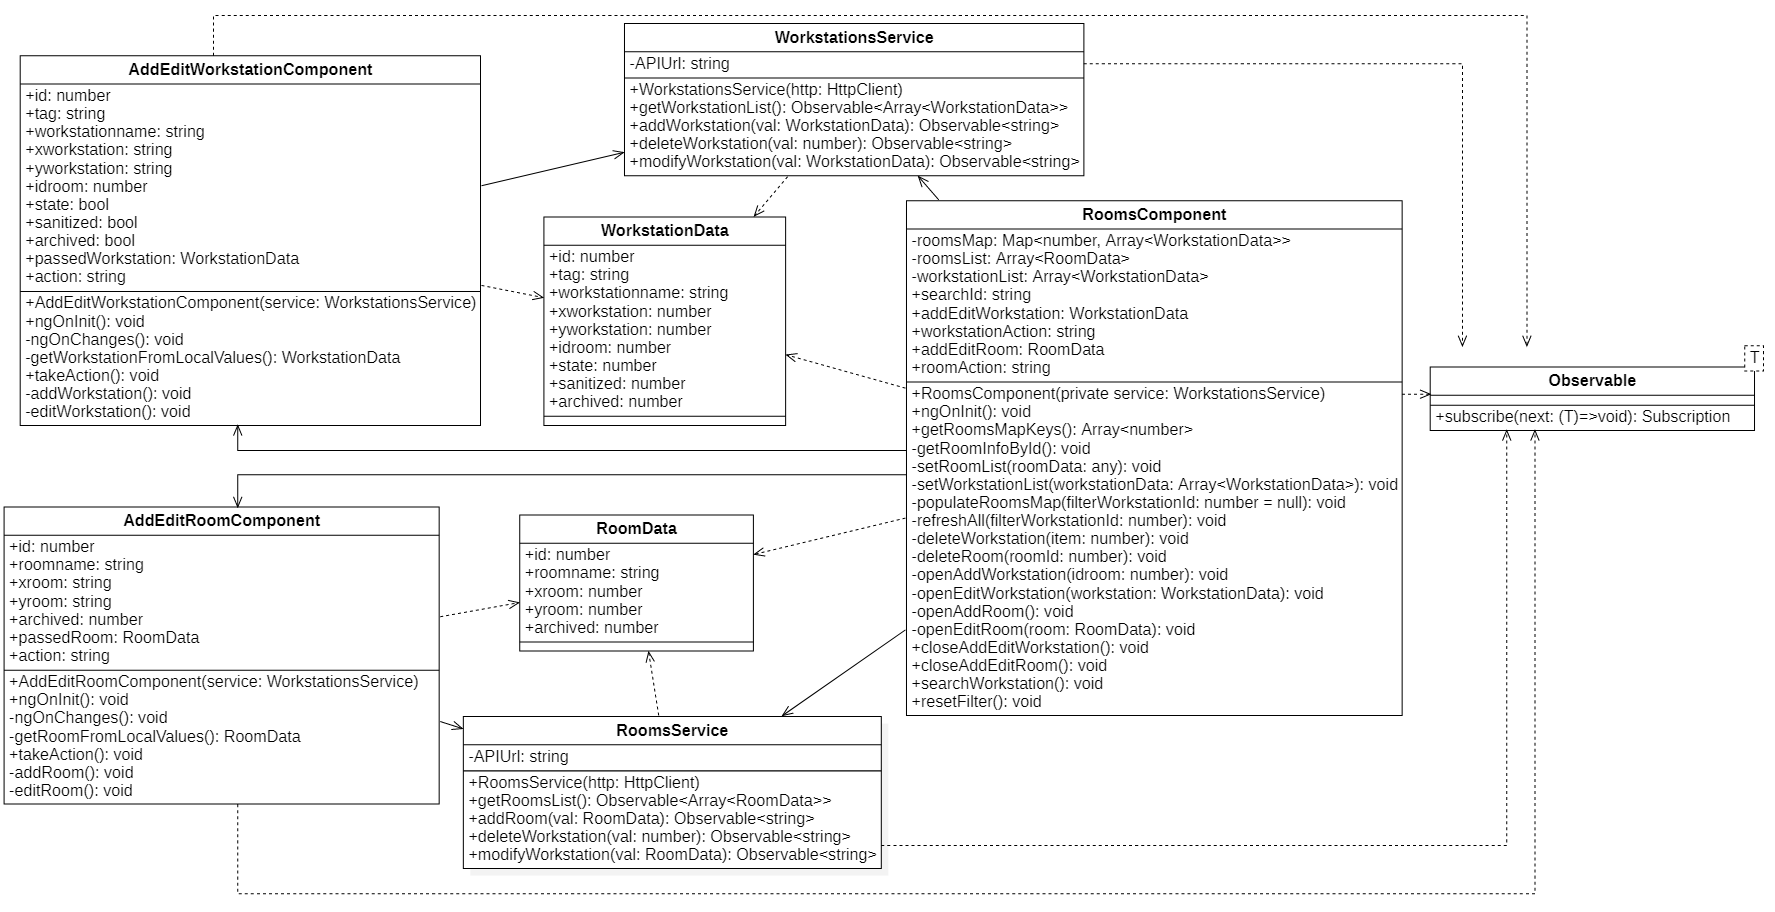
\includegraphics[width=18cm]{res/images/webapp-visualAddEditStanzePostazioni-diagrammaClassi.png}
	\caption{Diagramma delle classi per la gestione delle stanze e delle postazioni}
	\label{fig:DiagrammaClassiStanzePostazioni}
\end{figure}
Il diagramma sovrastante rappresenta l'architettura utilizzata per la pagina di gestione delle stanze e delle postazioni. \newline
\texttt{RoomsComponent} si occupa della visualizzazione ed eliminazione delle stanze e delle postazioni. Essa delega la creazione e modifica dei questi due dati alle classi \texttt{AddEditWorkstationComponent} e \texttt{AddEditRoomComponent}. Le tre componenti contengono un riferimento ad ognuno dei servizi di cui necessitano. I due servizi coinvolti sono \texttt{WorkstationService} e \texttt{RoomService}. Le informazini vengono ottenute dal server tramite la classe \texttt{Observable}. In generale i dati riguardanti postazioni e stanze sono scambiati utilizzando le due classi \texttt{WorkstationData} e \texttt{RoomData}.


\paragraph{Classi}
\subparagraph{RoomsComponent}
Classe che si occupa della visualizzazione, eliminazione e, tramite i componenti AddEditWorkstation e AddEditRoom, dell'aggiunta e modifica di postazioni e stanze. \newline
\textbf{Attributi}
\begin{itemize}
	\item \texttt{- roomsMap: Map<number, Array<WorkstationData>>} \newline
		Map in cui ad ogni stanza sono assegnate le sue postazione, ovvero quelle con \texttt{idroom} uguale all'\texttt{id} della stanza. Se l'utente applica un filtro alla lista, qui verranno contenute solo le stanze e le postazioni selezionate da tale filtro.
	\item \texttt{- roomsList: Array<RoomsData>} \newline
		Array utilizzato per contenere le stanze ottenutedal server
	\item \texttt{- workstationList: Array<Workstation>} \newline
		Array utilizzato per contenere le postazioni ottenute dal server.
	\item \texttt{+ searchId: string} \newline
		Id specificato dall'utente per la ricerca di una postazione.
	\item \texttt{+ addEditWorkstation: WorkstationData} \newline
		Contiene i dati della postazione che verrà aggiunta o modificata.
	\item \texttt{+ workstationAction: string} \newline
		Valore specificato dall'utente che provocherà la modifica o l'aggiunta della postazione salvata in \texttt{addEditWorkstation}
	\item \texttt{+ addEditRoom: RoomData} \newline
		Contiene i dati della stanza che verrà aggiunta o modificata.
	\item \texttt{+ roomAction: string} \newline
		Valore specificato dall'utente che provocherà la modifica o l'aggiunta della stanza salvata in \texttt{addEditRoom}
\end{itemize}
\textbf{Metodi}
\begin{itemize}
	\item \texttt{+ constructor(private service: SharedService, private cd: ChangeDetectorRef)} 
	\item \texttt{+ ngOnInit(): void} \newline
	Questa funzione viene chiamata all'inizializzazione della pagina.
	\item \texttt{+ getRoomsMapKeys(): Array<number>} \newline
	Restituisce un array con gli id delle stanze contenute in \texttt{roomsMap}
	\item \texttt{- getRoomInfoById(id: number): RoomData} \newline
	Restituisce un oggetto \texttt{RoomData} con i dati della stanza identificata dall'id passato come parametro.
	\item \texttt{- setRoomList(roomData: Array<RoomData>): void} \newline
	Reinizializza \texttt{roomList} con i dati ricevuti
	\item \texttt{- setWorkstationList(workstationData: Array<WorkstationData>): void} \newline
	Reinizializza \texttt{workstationList} con i dati ricevuti
	\item \texttt{- populateRoomsMap(filterWorkstationId: number): void} 
	Reinizializza \texttt{roomsMap} ponendo come chiavi gli id delle stanze contenute in \texttt{roomList} e come valori le postazioni contenute nelle rispettive stanze. \newline
	Se non viene specificato l'attributo \texttt{filterWorkstationId} nella mappa vengono inserite anche le stanze vuote. \newline
	Se viene specificato l'attributo \texttt{filterWorkstationId} verrà inserita nella mappa solo la postazione con l'id indicato e la stanza che la contiene.
	\item \texttt{- refreshAll(filterWorkstationId: number): void} \newline
	Richiede al server le stanze e le postazione e le organizza, tramite \texttt{populateRoomsMap}, in una mappa. Il parametro \texttt{filterWorkstationId} viene passato direttamente a \texttt{populateRoomsMap}
	\item \texttt{- deleteWorkstation(item: number): void} \newline
	Richiede al server l'eliminazione della postazione con l'id specificato
	\item \texttt{- deleteRoom(roomId: number): void} \newline
	Richiede al server l'eliminazione della stanza con l'id specificato
	\item \texttt{- openAddWorkstation(idroom: number): void} \newline
	Rende visibile il form per l'aggiunta di una postazione. Inoltre imposta i parametri necessari all'esecuzione di questa azione.
	\item \texttt{- openEditWorkstation(workstation: WorkstationData): void} \newline
	Rende visibile il form per la modifica di una postazione. Inoltre imposta i parametri necessari all'esecuzione di questa azione. 
	\item \texttt{- openAddRoom(): void} \newline
	Rende visibile il form per l'aggiunta di una stanza. Inoltre imposta i parametri necessari all'esecuzione di questa azione.
	\item \texttt{- openEditRoom(room: RoomData): void} \newline
	Rende visibile il form per la modifica di una stanza. Inoltre imposta i parametri necessari all'esecuzione di questa azione.
	\item \texttt{+ closeAddEditWorkstation(): void} \newline
	Provoca l'aggiornamento dei dati contenuti nella pagina.
	\item \texttt{+ closeAddEditRoom(): void} \newline
	Provoca l'aggiornamento dei dati contenuti nella pagina.
	\item \texttt{+ searchWorkstation(): void} \newline
	Richiede tutti i dati sulle postazioni e sulle stanze al server specificando il filtro indicato dall'utente.
	\item \texttt{+ resetFilter(): void} \newline
	Richiede tutti i dati sulle postazioni e sulle stanze al server senza alcun filtro.
\end{itemize}
	
\subparagraph{AddEditWorkstationComponent}
Classe che si occupa dell'aggiunta e modifica di postazioni. \newline
\textbf{Attributi}
\begin{itemize}
	\item \texttt{+ id: number } 
	\item \texttt{+ tag: string } 
	\item \texttt{+ workstationname: string } 
	\item \texttt{+ xworkstation: string } 
	\item \texttt{+ yworkstation: string } 
	\item \texttt{+ idroom: number } 
	\item \texttt{+ state: bool } 
	\item \texttt{+ sanitized: bool } 
	\item \texttt{+ archived: bool } 
	\item \texttt{+ passedWorkstation: WorkstationData } 
	\item \texttt{+ action: string} 
\end{itemize}
\textbf{Metodi}
\begin{itemize}
	\item \texttt{+ AddEditWorkstationComponent(service: WorkstationsService) }
	\item \texttt{+ ngOnInit(): void }
	\item \texttt{- ngOnChanges(): void }
	\item \texttt{- getWorkstationFromLocalValues(): WorkstationData }
	\item \texttt{+ takeAction(): void }
	\item \texttt{- addWorkstation(): void }
	\item \texttt{- editWorkstation(): void}
\end{itemize}
\subparagraph{AddEditRoomComponent}
Classe che si occupa dell'aggiunta e modifica di stanze. \newline
\textbf{Attributi}
\begin{itemize}
	\item \texttt{+ id: number 	}
	\item \texttt{+ roomname: string 	}
	\item \texttt{+ xroom: string 	}
	\item \texttt{+ yroom: string 	}
	\item \texttt{+ archived: number 	}
	\item \texttt{+ noticeChangeVariable: boolean 	}
	\item \texttt{+ passedRoom: RoomData 	}
	\item \texttt{+ action: string}
\end{itemize}
\textbf{Metodi}
\begin{itemize}
	\item \texttt{+ AddEditRoomComponent(service: WorkstationsService) 	}
	\item \texttt{+ ngOnInit(): void 	}
	\item \texttt{- ngOnChanges(): void 	}
	\item \texttt{- getRoomFromLocalValues(): RoomData 	}
	\item \texttt{+ takeAction(): void 	}
	\item \texttt{- addRoom(): void 	}
	\item \texttt{- editRoom(): void}
\end{itemize}
\subparagraph{WorkstationsService}
\textbf{Attributi}
\begin{itemize}
	\item \texttt{- APIUrl: string}
\end{itemize}
\textbf{Metodi}
\begin{itemize}
	\item \texttt{+ WorkstationsService(http: HttpClient) 	}
	\item \texttt{+ getWorkstationList(): Observable<Array<WorkstationData>> 	}
	\item \texttt{+ addWorkstation(val: WorkstationData): Observable<string> 	}
	\item \texttt{+ deleteWorkstation(val: number): Observable<string> 	}
	\item \texttt{+ modifyWorkstation(val: WorkstationData): Observable<string>}
\end{itemize}
\subparagraph{RoomsService}
\textbf{Attributi}
\begin{itemize}
	\item \texttt{- APIUrl: string}
\end{itemize}
\textbf{Metodi}
\begin{itemize}
	\item \texttt{+ RoomsService(http: HttpClient) 	}
	\item \texttt{+ getRoomsList(): Observable<Array<RoomData>> 	}
	\item \texttt{+ addRoom(val: RoomData): Observable<string> 	}
	\item \texttt{+ deleteWorkstation(val: number): Observable<string> 	}
	\item \texttt{+ modifyWorkstation(val: RoomData): Observable<string>}
\end{itemize}
\subparagraph{WorkstationData}
Classe che contiene tutti e soli i valori necessari per il salvataggio di una postazione sul database. È utilizzata per il transito dei dati delle postazioni all'interno dell'applicazione. \newline
\textbf{Attributi}
\begin{itemize}
	\item \texttt{+ id: number 	}
	\item \texttt{+ tag: string 	}
	\item \texttt{+ workstationname: string 	}
	\item \texttt{+ xworkstation: number 	}
	\item \texttt{+ yworkstation: number 	}
	\item \texttt{+ idroom: number 	}
	\item \texttt{+ state: number 	}
	\item \texttt{+ sanitized: number 	}
	\item \texttt{+ archived: number}
\end{itemize}
\subparagraph{RoomData}
Questa classe contiene tutti e soli i valori necessari per il salvataggio di una stanza sul database. È utilizzata per il transito dei dati delle stanze all'interno dell'applicazione. \newline
\textbf{Attributi}
\begin{itemize}
	\item \texttt{+ id: number 	}
	\item \texttt{+ roomname: string 	}
	\item \texttt{+ xroom: number 	}
	\item \texttt{+ yroom: number 	}
	\item \texttt{+ archived: number}
\end{itemize}
\subparagraph{Observable<T>}
Classe fornita dalla libreria Rxjs. Viene utilizzata per effettuare chiamate asincrone al server. Per una documnetazione più approfondita fare riferimento a \url{https://angular.io/guide/rx-library}. \newline
\textbf{Metodi}
\begin{itemize}
	\item \texttt{+ subscribe(next: (T)=>void): Subscription}
\end{itemize}

\subsubsection{Gestione credenziali}
\subsubsection{Sezione report}
\subsubsection{Sezione notifiche}
\subsection{Diagrammi di sequenza}
\subsubsection{Login}
\subsubsection{Gestione stanze e postazioni}
\begin{figure}[H]
	\centering
	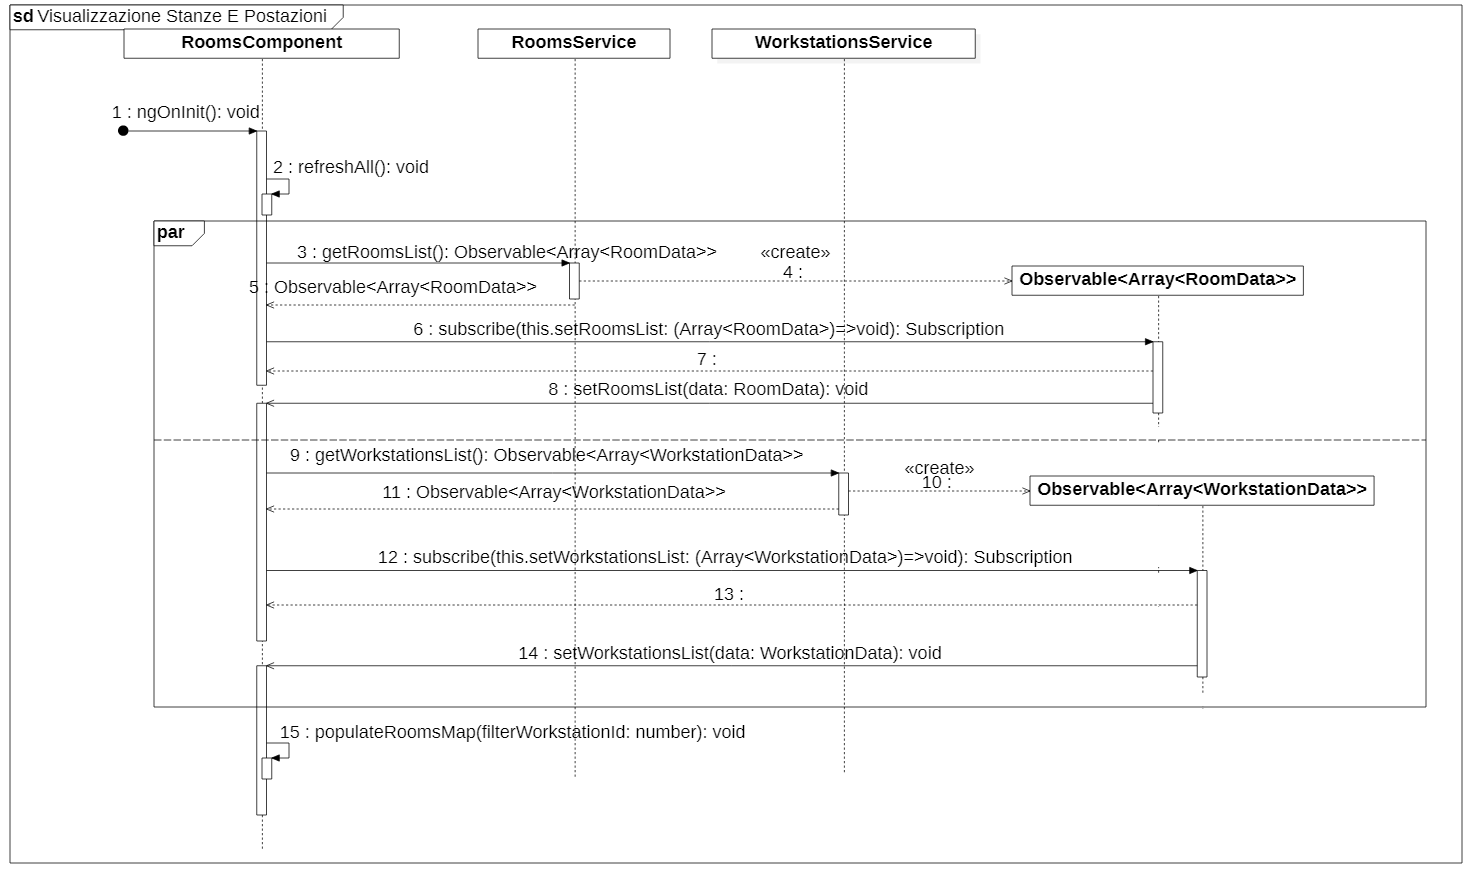
\includegraphics[width=18cm]{res/images/webapp-visualStanzePostazioni-diagrammaSequenza.png}
	\caption{Diagramma di sequenza per la visualizzazione delle stanze e delle postazioni}
	\label{fig:DiagrammaSequenzaStanzePostazioni1}
\end{figure}
Il diagramma sovrastante rappresenta un'evento scatenato dall'inizializzazione della pagina (notificata tramite la funzione \texttt{nfOnInit()}) che consiste nell'ottenimento di una lista delle postazioni e delle stanze dal server e della suddivisione delle prime in una mappa. Questa mappa verrà utilizzata dalla vista per mostrare le postazioni suddivise in stanze. L'evento rappresentato nel diagramma viene provocato ogni volta che si chiama il metodo \texttt{refreshAll()}. Questa funzionalità viene utilizzata, per esempio, dopo che una postazione è stata eliminata o modificata.
\begin{figure}[H]
	\centering
	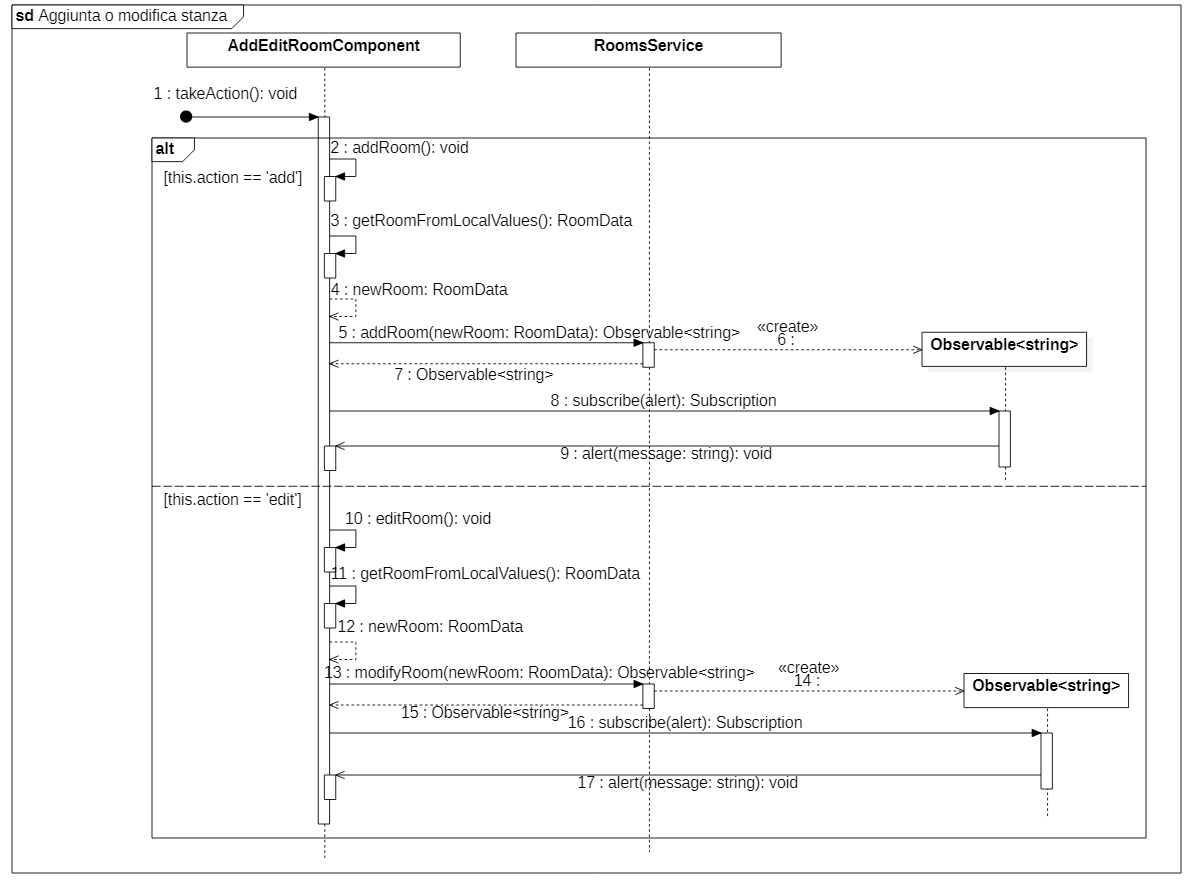
\includegraphics[width=18cm]{res/images/webapp-addEditStanzePostazioni-diagrammaSequenza.png}
	\caption{Diagramma di sequenza per l'aggiunta e la modifica di una stanza}
	\label{fig:DiagrammaSequenzaStanzePostazioni2}
\end{figure}
Il diagramma sovrastante rappresenta l'evento di aggiunta o modifica di una stanza.
In entrambi i casi l'evento è provocato dalla chiamata del metodo \texttt{takeAction()}, provocata dalla pressione di un pulsante da parte dell'utente. A questo punto la scelta dell'una o dell'altra via è determinata dal parametro \texttt{action}, che ha assunto valore 'add' o 'edit' a seconda del comportamento dell'utente.
\subsubsection{Gestione credenziali}
\subsubsection{Sezione report}
\subsubsection{Sezione notifiche}



